% Presentation : colonies de fourmis et voyageur de commerce
% Compilation : tectonic presentation.tex   (ou xelatex / lualatex)
\documentclass[aspectratio=169,11pt]{beamer}

\usetheme[progressbar=frametitle,numbering=fraction]{metropolis}
\usepackage[french]{babel}
\usepackage{amsmath,amssymb}
\usepackage{booktabs}
\usepackage{tikz}
\usetikzlibrary{babel,arrows.meta,positioning}

\graphicspath{{figures/}{../results/figures/}}

\definecolor{acoblue}{HTML}{2A78D6}
\definecolor{acoorange}{HTML}{EB6834}
\definecolor{acogreen}{HTML}{1BAF7A}
\setbeamercolor{alerted text}{fg=acoorange}
\newcommand{\bon}[1]{\textcolor{acogreen}{\textbf{#1}}}

\title{Colonies de fourmis et problème du voyageur de commerce}
\subtitle{Précision contre temps de calcul : quand utiliser l'ACO ?}
\author{Ivano Balboni \and Quentin Wache}
\date{Novembre 2026}

\begin{document}

\maketitle

% ------------------------------------------------------------
\begin{frame}{Plan}
  \begin{columns}[T]
    \column{0.5\textwidth}
    \begin{enumerate}
      \item Le problème et les méthodes classiques
      \item Le modèle ACO
      \item Ce que prédit la théorie
      \item Protocole expérimental
    \end{enumerate}
    \column{0.5\textwidth}
    \begin{enumerate}\setcounter{enumi}{4}
      \item Complexité : mesure vs théorie
      \item Précision vs temps de calcul
      \item Cas d'usage et limites
    \end{enumerate}
  \end{columns}
  \vspace{1em}
  \alert{Question centrale :} pour un temps de calcul donné, quel algorithme donne la
  meilleure tournée, et l'ACO a-t-il sa place ?
\end{frame}

% ============================================================
\section{Le problème}
% ============================================================

\begin{frame}{Le voyageur de commerce (TSP)}
  \begin{columns}[c]
    \column{0.55\textwidth}
    \begin{itemize}
      \item $n$ villes, distances $d_{ij}$
      \item Trouver le \alert{cycle le plus court} qui passe une fois par chaque ville
      \item Problème \alert{NP-difficile} : aucun algorithme polynomial connu
      \item Nombre de tournées distinctes : $\dfrac{(n-1)!}{2}$
    \end{itemize}
    \column{0.42\textwidth}
    \centering
    \begin{tabular}{rr}
      \toprule
      $n$ & tournées possibles \\
      \midrule
      10  & $1{,}8 \times 10^{5}$ \\
      20  & $6{,}1 \times 10^{16}$ \\
      30  & $4{,}4 \times 10^{30}$ \\
      50  & $3{,}0 \times 10^{62}$ \\
      100 & $4{,}7 \times 10^{155}$ \\
      \bottomrule
    \end{tabular}
  \end{columns}
  \vspace{0.8em}
  \small À un milliard de tournées par seconde, $n = 20$ prend déjà \alert{2 ans}.
  Il faut donc choisir entre \alert{exactitude} et \alert{temps de calcul}.
\end{frame}

\begin{frame}{Les algorithmes comparés}
  \centering
  \footnotesize
  \begin{tabular}{llll}
    \toprule
    Algorithme & Famille & Complexité théorique & Garantie \\
    \midrule
    Held-Karp & exact (prog. dynamique) & $O(n^2 2^n)$ & optimum \\
    Plus proche voisin (PPV) & glouton & $O(n^2)$ & aucune \\
    PPV + 2-opt & recherche locale & $O(n^2)$ par passe & optimum local \\
    Christofides & approximation & $O(n^3)$ & $\le 1{,}5 \times$ optimum \\
    Recuit simulé & métaheuristique & $O(\text{itérations})$ & asymptotique \\
    OR-Tools (Google) & solveur industriel & limite de temps & aucune \\
    \midrule
    ACO (AS, ACS, MMAS) & métaheuristique & $O(T\,m\,n^2)$ & asymptotique \\
    ACO MMAS + 2-opt & hybride & $O(T\,m\,n^2)$ + 2-opt & asymptotique \\
    \bottomrule
  \end{tabular}

  \vspace{0.6em}
  \raggedright
  $T$ : itérations, $m$ : fourmis. Témoin ajouté : \alert{2-opt multi-départs}
  (2-opt relancé depuis des tournées aléatoires), pour isoler l'apport de l'apprentissage.
\end{frame}

% ============================================================
\section{Le modèle ACO}
% ============================================================

\begin{frame}{Inspiration : l'expérience du double pont}
  \begin{columns}[c]
    \column{0.48\textwidth}
    \centering
    \begin{tikzpicture}[scale=1.0, every node/.style={font=\small}]
      \node[circle, fill=acoblue!20, draw=acoblue, minimum size=1.1cm] (nid) at (0,0) {Nid};
      \node[circle, fill=acoorange!20, draw=acoorange, minimum size=1.1cm] (food) at (5,0) {Nourriture};
      \draw[line width=4pt, acoblue] (nid) to[out=40, in=140] node[above] {court} (food);
      \draw[line width=1pt, gray] (nid) to[out=-70, in=-110] node[below] {long} (food);
    \end{tikzpicture}
    \column{0.5\textwidth}
    \begin{itemize}
      \item Les fourmis déposent une \alert{phéromone} sur leur chemin
      \item Sur le chemin court, les allers-retours sont plus rapides
            $\Rightarrow$ plus de dépôt
      \item Plus de phéromone $\Rightarrow$ plus de fourmis : \alert{rétroaction positive}
      \item L'évaporation efface les mauvais chemins
    \end{itemize}
    \small Deneubourg et al. (1990) ; communication indirecte par l'environnement = \emph{stigmergie}
  \end{columns}
\end{frame}

\begin{frame}{Ant System (Dorigo et al., 1996)}
  À chaque itération, $m$ fourmis construisent chacune une tournée.

  \medskip
  \textbf{1. Choix de la ville suivante} (fourmi $k$ en $i$, villes non visitées $\mathcal{N}_k$) :
  \[
    p_{ij} = \frac{\tau_{ij}^{\,\alpha}\;\eta_{ij}^{\,\beta}}
                  {\sum_{l \in \mathcal{N}_k} \tau_{il}^{\,\alpha}\;\eta_{il}^{\,\beta}}
    \qquad \eta_{ij} = \frac{1}{d_{ij}}
  \]

  \textbf{2. Mise à jour des phéromones} (après toutes les fourmis) :
  \[
    \tau_{ij} \leftarrow \underbrace{(1-\rho)\,\tau_{ij}}_{\text{évaporation}}
              + \underbrace{\sum_{k} \frac{Q}{L_k}\,\mathbb{1}[(i,j) \in T_k]}_{\text{dépôt}}
  \]

  \begin{columns}[T]
    \column{0.5\textwidth}
    \small
    $\alpha$ : poids de la mémoire collective \\
    $\beta$ : poids de la distance (glouton)
    \column{0.5\textwidth}
    \small
    $\rho$ : vitesse d'oubli \\
    $m$ : nombre de fourmis, $L_k$ : longueur de la tournée $k$
  \end{columns}
\end{frame}

\begin{frame}{Démonstration}
  \begin{columns}[c]
    \column{0.6\textwidth}
    \centering
    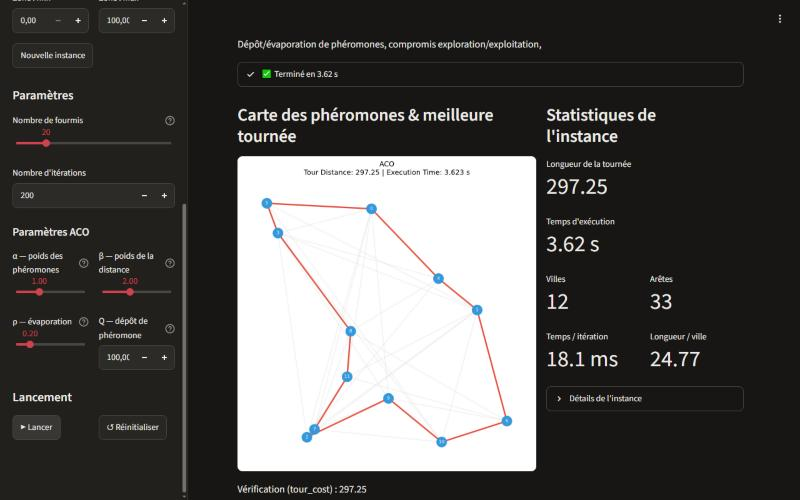
\includegraphics[width=\textwidth]{demo_streamlit.png}
    \column{0.37\textwidth}
    \small
    \textbf{En direct, 20 villes :}
    \begin{enumerate}
      \item Réglages de référence : $\alpha = 1$, $\beta = 2$, $\rho = 0{,}2$
      \item $\alpha = 3$ : la colonie se fige sur une piste trop tôt
      \item $\beta = 0$ : sans la distance, presque du hasard
    \end{enumerate}
    \medskip
    \tiny
    \href{https://using-aco-for-tsp-faqcu8kd7htkggervtpugk.streamlit.app}{\texttt{using-aco-for-tsp-faqcu8kd7htkggervtpugk}\\\texttt{.streamlit.app}}
  \end{columns}
\end{frame}

\begin{frame}{Variantes testées}
  \begin{description}[MMAS + 2-opt]
    \item[AS] Ant System : toutes les fourmis déposent
    \item[ACS] Ant Colony System (Dorigo \& Gambardella, 1997) : avec probabilité $q_0 = 0{,}9$,
               choix de la meilleure arête ; mise à jour locale pendant la construction
    \item[MMAS] MAX-MIN Ant System (Stützle \& Hoos, 2000) : seule la meilleure fourmi dépose,
                $\tau \in [\tau_{\min}, \tau_{\max}]$ avec $\tau_{\max} = \frac{1}{\rho L^{*}}$,
                réinitialisation si la colonie stagne
    \item[+ 2-opt] Recherche locale appliquée aux meilleures tournées de chaque itération
  \end{description}
  \vspace{0.5em}
  \begin{block}{Point commun}
    Ce sont des algorithmes \alert{anytime} : on peut les arrêter à tout moment, et la
    solution s'améliore avec le temps accordé.
  \end{block}
\end{frame}

% ============================================================
\section{Ce que prédit la théorie}
% ============================================================

\begin{frame}{Complexité d'une itération d'ACO}
  \begin{columns}[T]
    \column{0.55\textwidth}
    \begin{itemize}
      \item Construction : $m$ fourmis $\times$ $(n-1)$ pas $\times$ $O(n)$ candidats
            \[ \Rightarrow O(m\,n^2) \]
      \item Évaporation $O(n^2)$, dépôt $O(m\,n)$
      \item Total pour $T$ itérations : $\boxed{O(T\,m\,n^2)}$
      \item Mémoire : matrice des phéromones $O(n^2)$
    \end{itemize}
    \column{0.42\textwidth}
    \begin{block}{Prédictions testables}
      \begin{itemize}
        \item $m$ et $T$ fixés : temps $\propto n^2$ \\ (pente 2 en log-log)
        \item Ajouter 2-opt : chaque passe coûte $O(n^2)$, et le nombre de passes croît avec $n$
        \item Held-Karp : temps $\times \approx 2$ par ville ajoutée
      \end{itemize}
    \end{block}
  \end{columns}
\end{frame}

\begin{frame}{Dynamique des phéromones et convergence}
  \textbf{Évaporation seule :} $\tau_t = \tau_0 (1-\rho)^t$ \\
  \quad $\Rightarrow$ la colonie \og oublie\fg{} en environ $1/\rho$ itérations
  \quad ($\rho = 0{,}2$ : 5 it. ; $\rho = 0{,}02$ : 50 it.)

  \smallskip
  \textbf{Dépôt constant $\Delta$ :} $\tau_t \to \Delta / \rho$ (point fixe)

  \smallskip
  \textbf{Résultats de convergence}
  \begin{itemize}\small
    \item Gutjahr (2000) : un Ant System modifié trouve l'optimum avec une probabilité qui tend vers 1
    \item Stützle \& Dorigo (2002) : avec $\tau_{\min} > 0$, la probabilité de trouver l'optimum tend vers 1
  \end{itemize}

  \begin{alertblock}{Mais}
    Garanties \alert{asymptotiques} uniquement : aucun temps polynomial (le TSP est NP-difficile).
    La vraie question est donc expérimentale : \alert{quelle précision pour quel temps ?}
  \end{alertblock}
\end{frame}

% ============================================================
\section{Protocole expérimental}
% ============================================================

\begin{frame}{Protocole}
  \footnotesize
  \begin{columns}[T]
    \column{0.5\textwidth}
    \textbf{Expérience 1 : complexité}
    \begin{itemize}
      \item Instances aléatoires, $n = 25$ à $800$
      \item Held-Karp : $n = 6$ à $16$
      \item ACO : 25 fourmis, 10 itérations
      \item Pente mesurée en log-log sur les grands $n$
    \end{itemize}
    \textbf{Expérience 2 : précision vs temps}
    \begin{itemize}
      \item TSPLIB à \alert{optimum prouvé} : eil51, kroA100, ch150
      \item Budget de 30 s, 3 graines par algorithme aléatoire
      \item On enregistre la meilleure tournée au cours du temps
    \end{itemize}
    \column{0.5\textwidth}
    \textbf{Trois types d'algorithmes}
    \begin{itemize}
      \item \emph{Un coup} (un point) : PPV, PPV + 2-opt, Christofides
      \item \emph{Budget réglable} : recuit simulé (30 à 30\,000 $n$ itérations),
            OR-Tools (0,1 à 30 s)
      \item \emph{Anytime} (une courbe) : ACO, 2-opt multi-départs
    \end{itemize}
    \textbf{Équité}
    \begin{itemize}
      \item Tous les algorithmes sur \alert{un seul cœur} de la même machine
      \item Même budget de temps pour tous
      \item Paramètres standards de la littérature, sans réglage par instance
    \end{itemize}
  \end{columns}
\end{frame}

% ============================================================
\section{Complexité : mesure vs théorie}
% ============================================================

\begin{frame}{Temps de calcul en fonction de $n$}
  \centering
  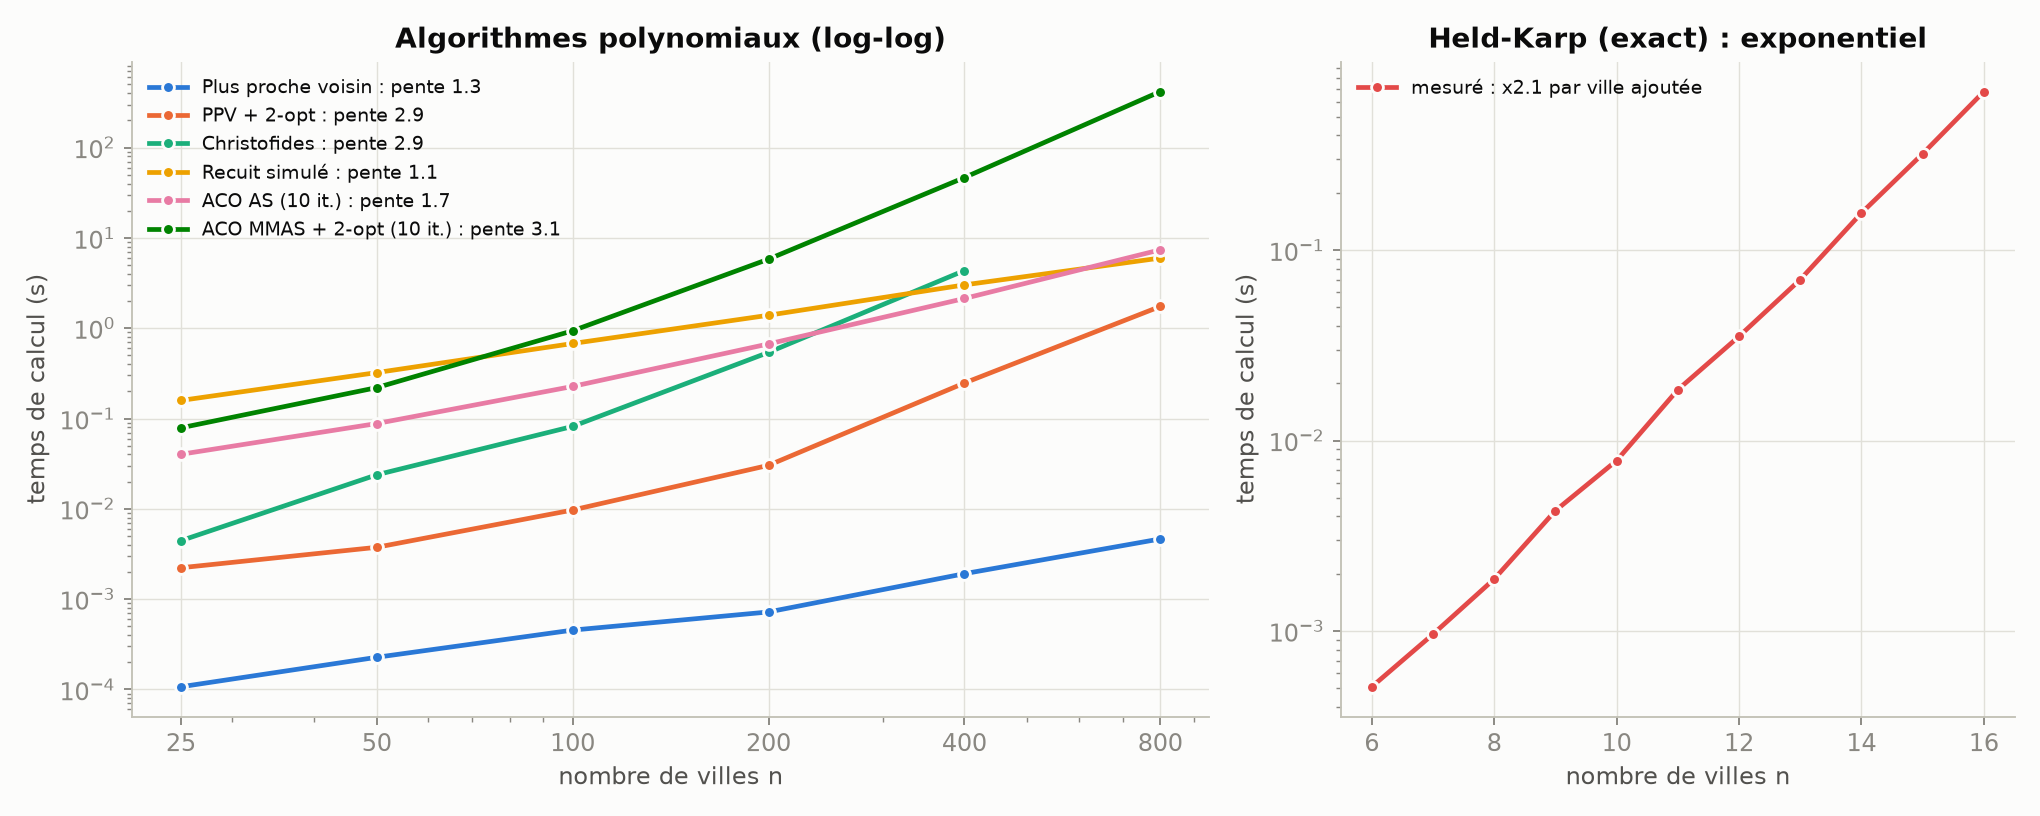
\includegraphics[width=\textwidth]{complexity_all.png}
\end{frame}

\begin{frame}{Pentes mesurées vs théorie}
  \centering
  \small
  \begin{tabular}{lccl}
    \toprule
    Algorithme & Théorie & Mesuré & Lecture \\
    \midrule
    Christofides & 3 & \bon{2,9} & conforme \\
    PPV + 2-opt & $\approx 3$ & \bon{2,9} & $O(n^2)$ par passe $\times$ $O(n)$ passes \\
    ACO AS ($m$, $T$ fixés) & 2 & 1,7 & proche, coûts fixes par pas \\
    ACO MMAS + 2-opt & $> 2$ & 3,1 & dominé par le 2-opt \\
    Plus proche voisin & 2 & 1,3 & boucle interne vectorisée \\
    Recuit simulé & 1 à 2 & 1,1 & coût par itération quasi constant \\
    Held-Karp & $\times 2{,}3$ / ville & \bon{$\times$ 2,1} & exponentiel, conforme \\
    \bottomrule
  \end{tabular}

  \vspace{0.3em}
  \raggedright
  \begin{itemize}\footnotesize
    \item Les écarts viennent des \alert{coûts fixes} de l'implémentation : une opération sur $n$
          valeurs coûte presque autant pour $n = 25$ que pour $n = 800$. La théorie décrit le
          comportement pour $n$ grand.
    \item Held-Karp : 0,7 s à $n = 16$ ; extrapolé à $n = 30$ : $\approx 6$ h et
          \alert{plus de 100 Go} de mémoire.
  \end{itemize}
\end{frame}

% ============================================================
\section{Précision vs temps de calcul}
% ============================================================

\begin{frame}{kroA100 : précision en fonction du temps accordé}
  \centering
  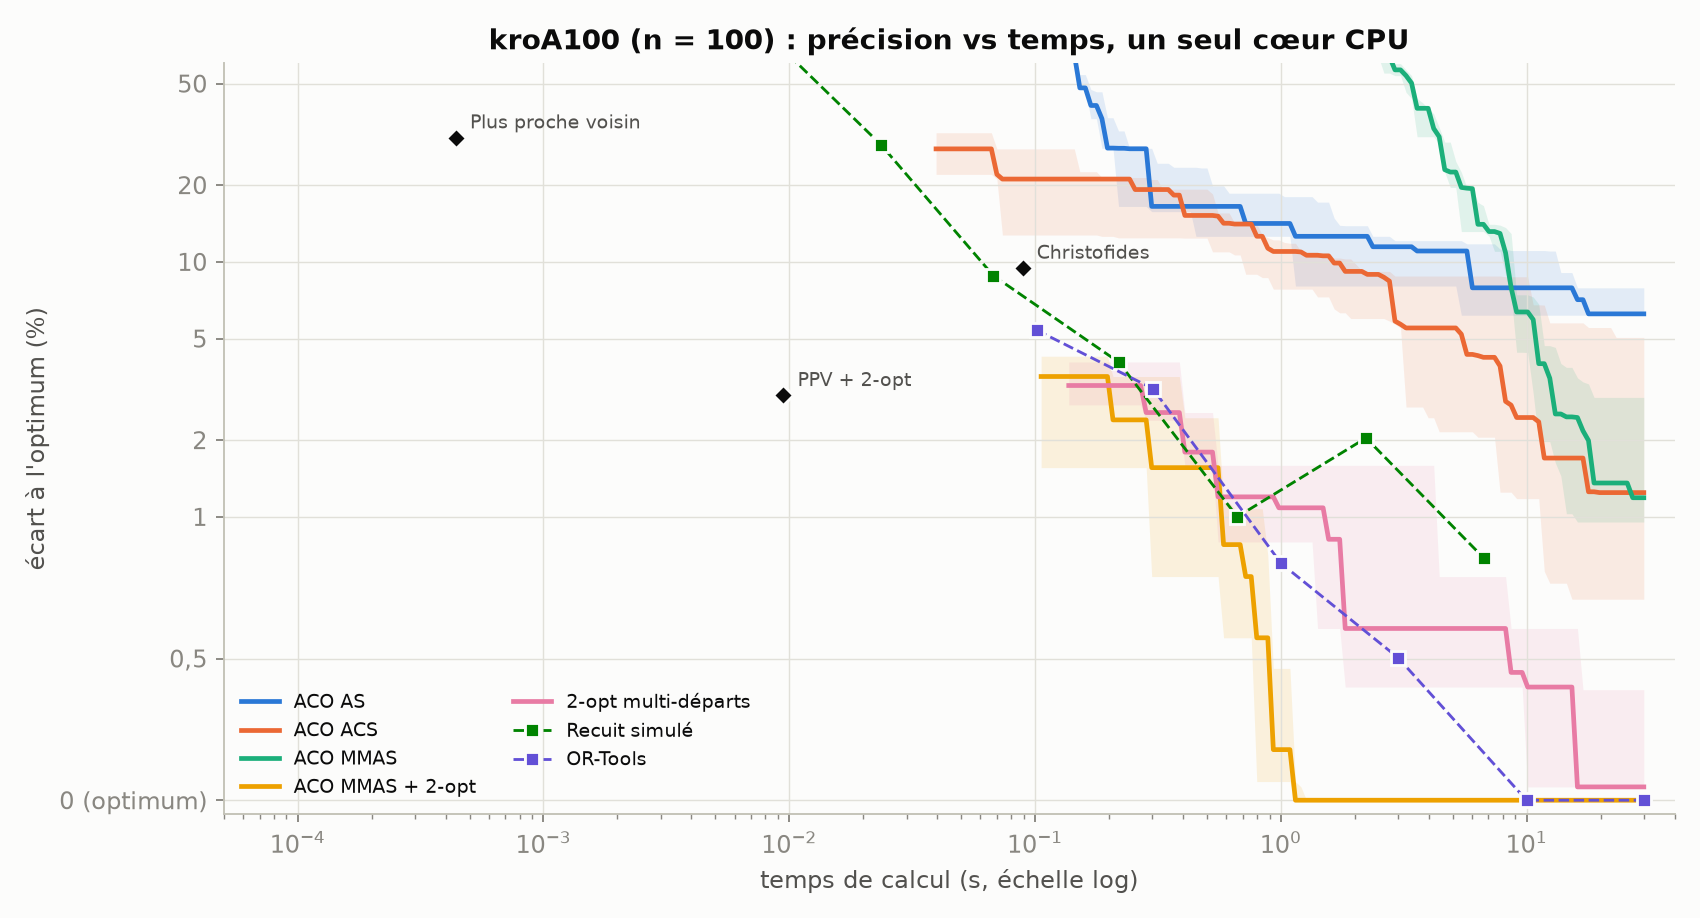
\includegraphics[height=0.84\textheight]{anytime_kroA100.png}
\end{frame}

\begin{frame}{ch150 : précision en fonction du temps accordé}
  \centering
  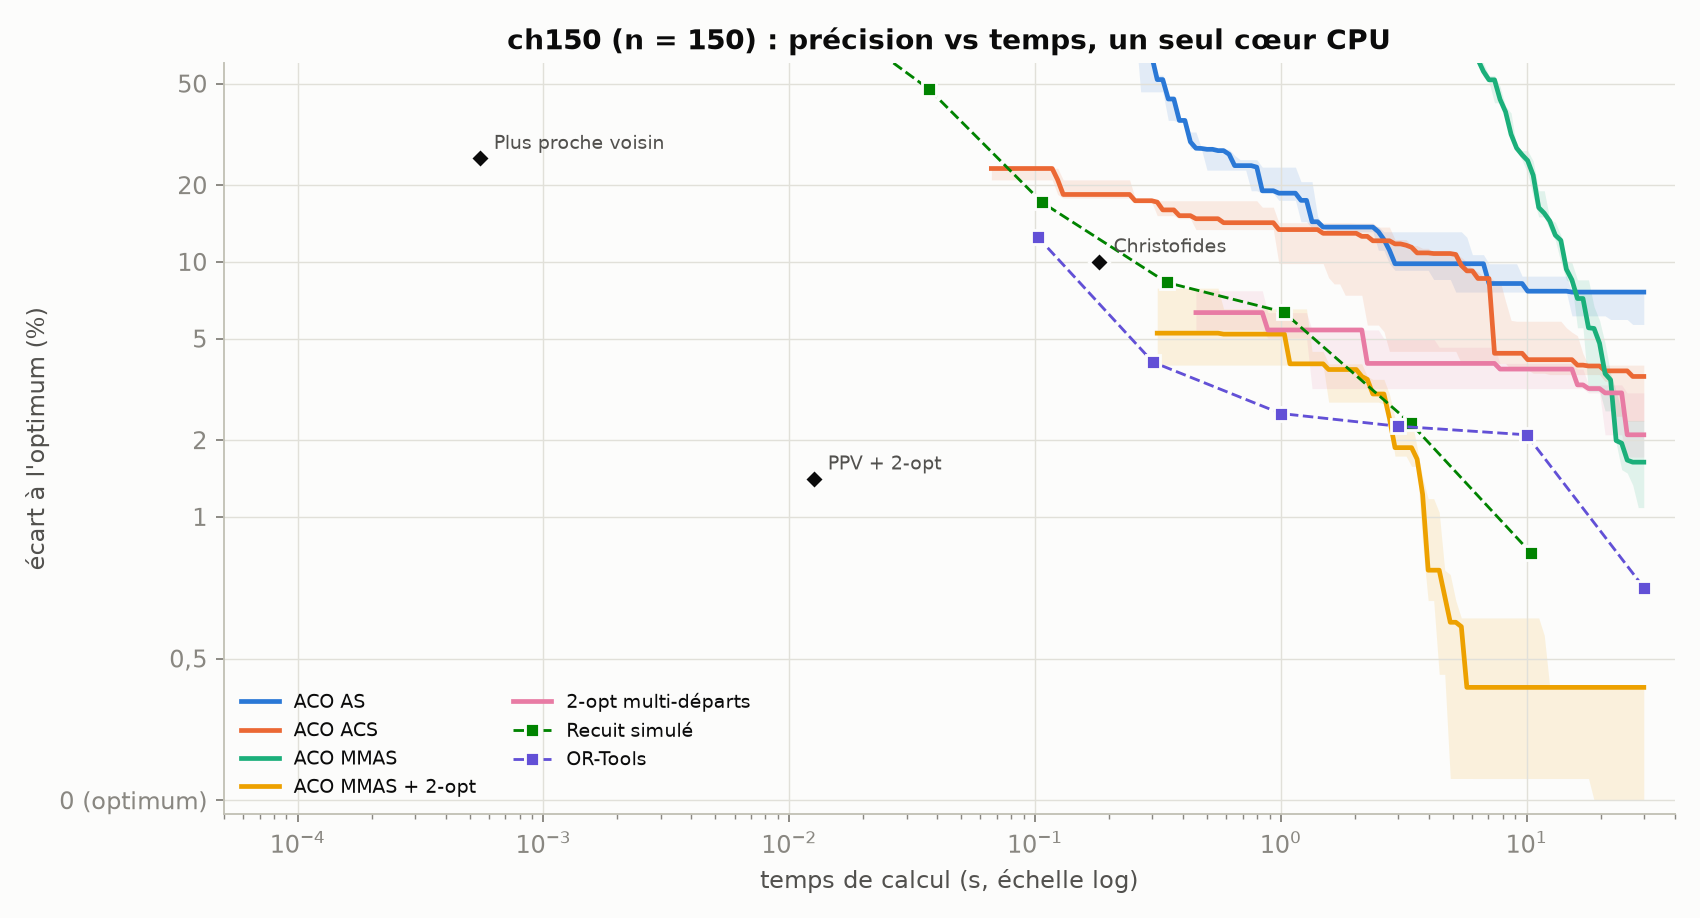
\includegraphics[height=0.84\textheight]{anytime_ch150.png}
\end{frame}



\begin{frame}{Quel algorithme gagne, selon le temps disponible ?}
  \centering
  \footnotesize
  \begin{tabular}{llll}
    \toprule
    Budget & eil51 ($n = 51$) & kroA100 ($n = 100$) & ch150 ($n = 150$) \\
    \midrule
    10 ms  & PPV+2-opt (2,1 \%) & PPV+2-opt (3,0 \%) & PPV+2-opt$^{*}$ (1,4 \%) \\
    0,1 s  & PPV+2-opt (2,1 \%) & PPV+2-opt (3,0 \%) & PPV+2-opt (1,4 \%) \\
    1 s    & \alert{MMAS+2-opt} (0,1 \%) & \alert{MMAS+2-opt} (0,2 \%) & PPV+2-opt (1,4 \%) \\
    10 s   & \alert{MMAS+2-opt} (0,1 \%) & \alert{MMAS+2-opt}$^{\dagger}$ (0 \%) & \alert{MMAS+2-opt} (0,4 \%) \\
    30 s   & \alert{MMAS+2-opt}$^{\ddagger}$ (0,1 \%) & \alert{MMAS+2-opt}$^{\dagger}$ (0 \%) & \alert{MMAS+2-opt} (0,3 \%) \\
    \bottomrule
  \end{tabular}

  \raggedright\scriptsize $^{*}$ en 13 ms ; $^{\dagger}$ ex æquo avec OR-Tools ;
  $^{\ddagger}$ ex æquo avec 2-opt multi-départs. \normalsize
  \vspace{0.5em}
  \raggedright
  \begin{itemize}
    \item Temps très court : \alert{PPV + 2-opt} est imbattable
    \item Dès que le budget permet plusieurs centaines d'itérations, \alert{MMAS + 2-opt} prend la
          tête ; le seuil augmente avec $n$ ($< 1$ s pour 100 villes, $\approx 4$ s pour 150)
    \item Les ACO \alert{sans} recherche locale ne gagnent jamais
  \end{itemize}
\end{frame}

\begin{frame}{L'apprentissage des fourmis sert-il vraiment ?}
  \begin{columns}[c]
    \column{0.5\textwidth}
    \textbf{Contre le hasard} (30 villes, 2\,000 tournées)
    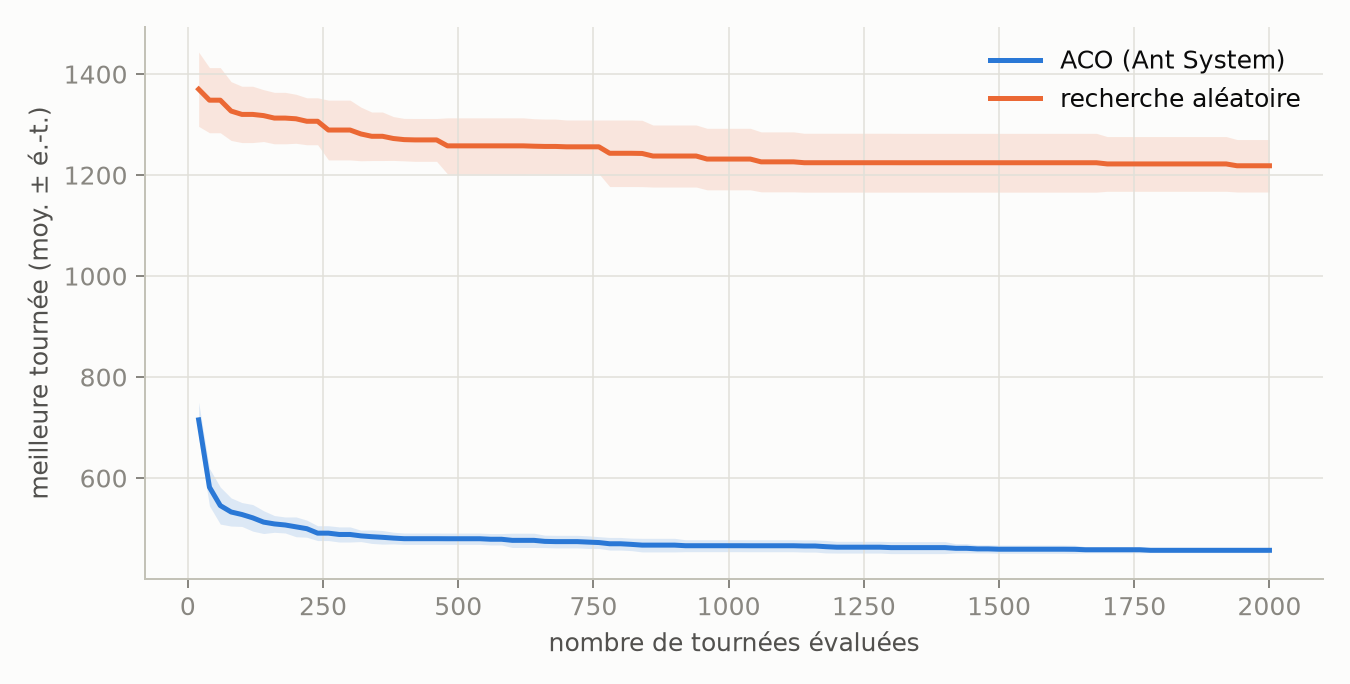
\includegraphics[width=\textwidth]{aco_vs_random.png}
    \small ACO : \bon{457} ; recherche aléatoire : 1218
    \column{0.47\textwidth}
    \textbf{Contre le témoin 2-opt multi-départs}
    \footnotesize
    \begin{center}
    \setlength{\tabcolsep}{4pt}
    \begin{tabular}{lrr}
      \toprule
      à 10 s (\%) & 2-opt m.-d. & MMAS+2-opt \\
      \midrule
      eil51   & 0,55 & \bon{0,08} \\
      kroA100 & 0,35 & \bon{0,00} \\
      ch150   & 3,66 & \bon{0,37} \\
      \bottomrule
    \end{tabular}
    \end{center}
    Même recherche locale, même temps : partir des tournées proposées par les fourmis
    plutôt que de tournées aléatoires divise l'écart par \alert{7 à 10}, et atteint l'optimum
    sur kroA100.
  \end{columns}
\end{frame}

\begin{frame}{Paramètres : le compromis précision/temps dans l'ACO lui-même}
  \centering
  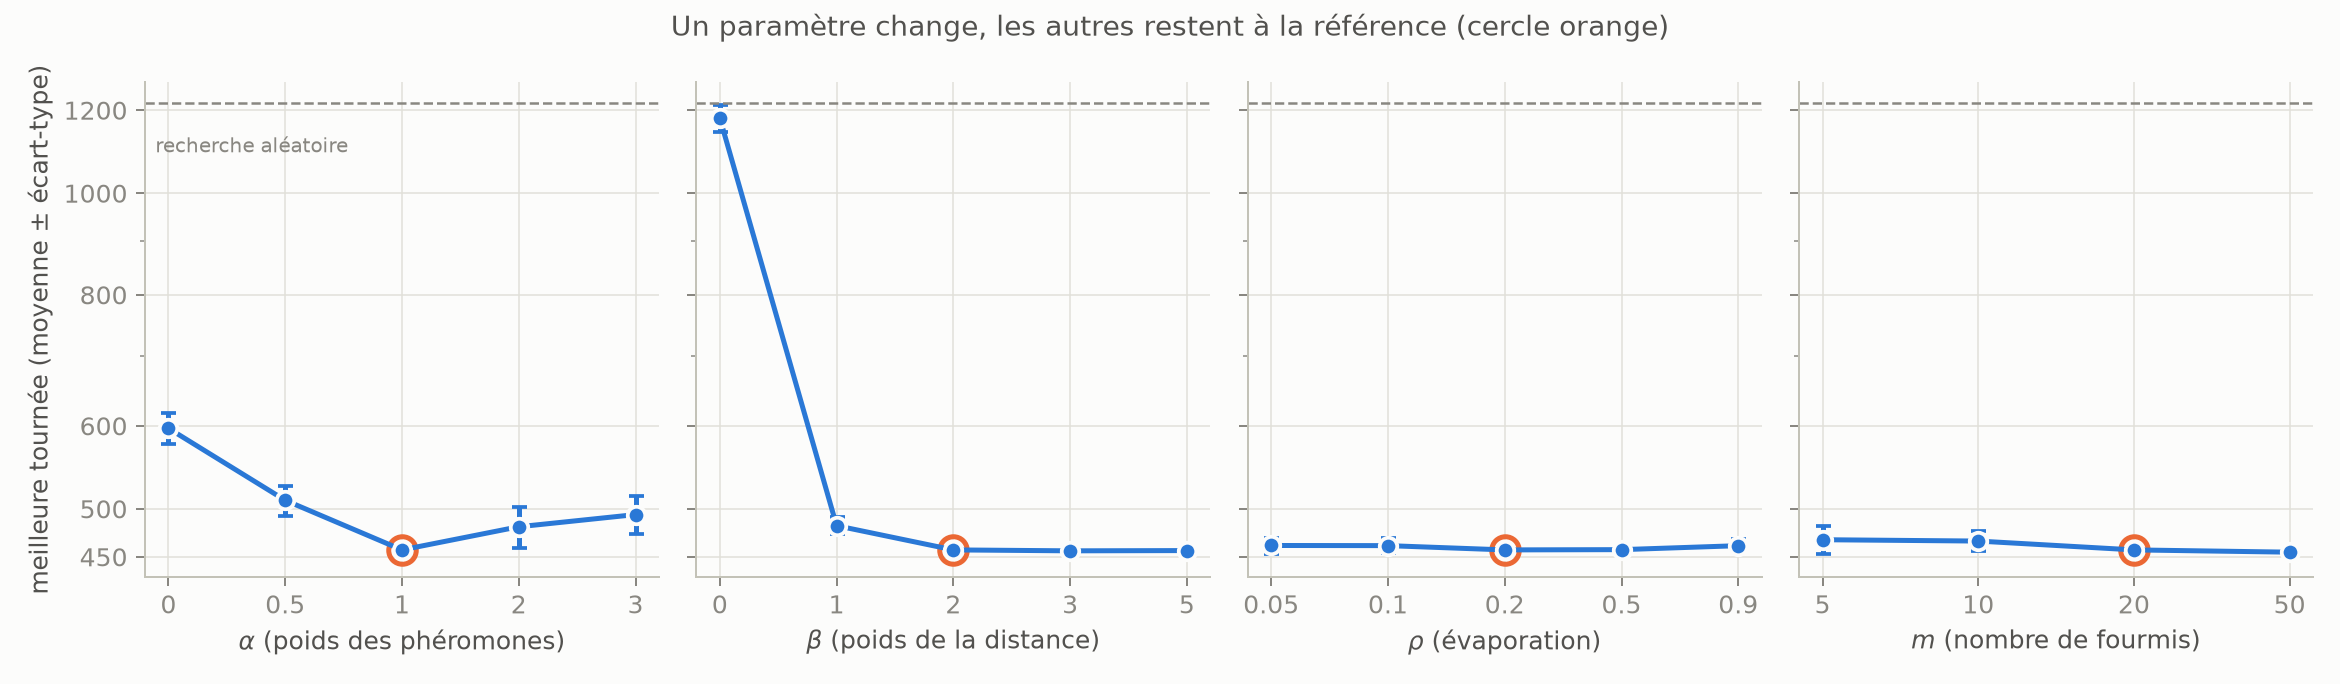
\includegraphics[height=0.40\textheight]{params_effect.png}
  \vspace{-0.4em}
  \begin{columns}[c]
    \column{0.42\textwidth}
    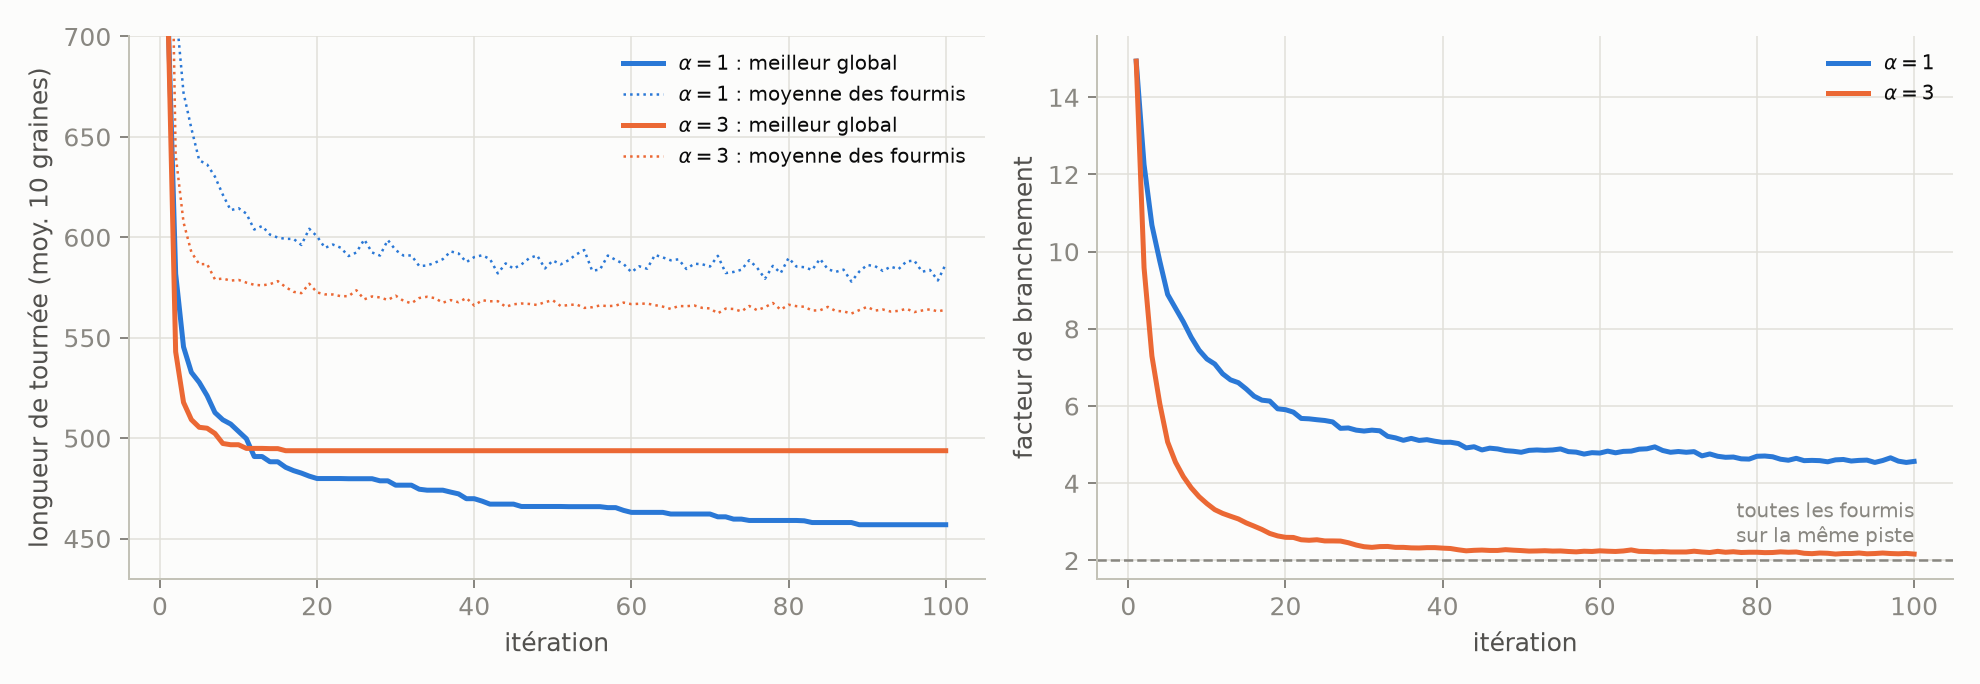
\includegraphics[width=\textwidth,height=0.36\textheight,keepaspectratio]{premature.png}
    \column{0.56\textwidth}
    \footnotesize
    \begin{itemize}
      \item $\alpha = 3$ : converge en $\approx 10$ it. mais s'arrête à $494$ ;
            $\alpha = 1$ : $\approx 40$ it., atteint $457$
      \item $\beta = 0$ : presque le hasard ; $\alpha = 0$ (pas de mémoire) : $597$
      \item $\rho$ : peu d'effet ; plus de fourmis : plus régulier (é.-t. 14,6 $\to$ 1,1)
    \end{itemize}
    \scriptsize 30 villes, 10 graines. Détail : page \og Analyse\fg{} de la démo.
  \end{columns}
\end{frame}

% ============================================================
\section{Cas d'usage et limites}
% ============================================================

\begin{frame}{Quel algorithme pour quelle situation ? (TSP statique)}
  \centering
  \footnotesize
  \begin{tabular}{p{3.9cm}p{2.6cm}p{5.6cm}}
    \toprule
    Situation & Choix & Justification mesurée \\
    \midrule
    $n \le 15$, optimum exigé & Held-Karp & exact en $< 1$ s ; $\times 2$ par ville ensuite \\
    Réponse en quelques ms & PPV + 2-opt & 1,4 à 3 \% en 3 à 13 ms \\
    Garantie théorique exigée & Christofides & $\le 1{,}5\times$ prouvé ; mesuré 8 à 10 \% \\
    Quelques secondes, meilleure qualité & \textcolor{acoorange}{MMAS + 2-opt} & 0 à 0,4 \% en 10 s ; optimum sur kroA100 \\
    Solveur prêt à l'emploi & OR-Tools & 0 à 0,8 \% en 30 s, sans réglage \\
    ACO sans recherche locale & à éviter & 0,4 à 7 \% en 30 s ; toujours battu par une méthode avec 2-opt \\
    \bottomrule
  \end{tabular}

  \vspace{0.6em}
  \raggedright\small
  L'ACO joue le rôle de \alert{générateur de bons points de départ} pour la recherche locale.
\end{frame}

\begin{frame}{Où l'ACO a un avantage structurel}
  \begin{columns}[T]
    \column{0.5\textwidth}
    \textbf{Problèmes qui changent dans le temps}
    \begin{itemize}
      \item Routage réseau (AntNet, Di Caro \& Dorigo, 1998) : les phéromones s'adaptent quand les
            coûts changent, sans tout recalculer
    \end{itemize}
    \textbf{Problèmes avec contraintes métier}
    \begin{itemize}
      \item Tournées de véhicules (capacités, créneaux), ordonnancement d'ateliers, affectation
            quadratique
      \item La contrainte s'ajoute dans la règle de choix de la fourmi
    \end{itemize}
    \column{0.5\textwidth}
    \begin{alertblock}{Où ce n'est pas utile}
      Plus court chemin sur un graphe fixe : Dijkstra est exact en
      $O((V+E)\log V)$. Une métaheuristique ne se justifie que si le problème est
      NP-difficile ou change dans le temps.
    \end{alertblock}
    \begin{block}{Coût à prévoir}
      Réglage des paramètres ($\alpha$, $\beta$, $\rho$) et quelques secondes de calcul
      avant de battre les heuristiques simples.
    \end{block}
  \end{columns}
\end{frame}

\begin{frame}{Limites de notre étude}
  \begin{itemize}
    \item Trois instances TSPLIB, $n \le 150$ : le seuil où MMAS + 2-opt devient le meilleur
          choix augmente avec $n$ et reste à mesurer au-delà
    \item Budget maximal de 30 s, sur une seule machine
    \item Paramètres standards de la littérature, non réglés par instance (ni pour l'ACO, ni pour
          le recuit simulé, ni pour OR-Tools)
    \item Implémentation Python : les temps absolus seraient plus faibles en C, mais les pentes
          et le classement devraient rester proches
    \item Les avantages \og dynamique\fg{} et \og contraintes\fg{} de l'ACO viennent de la
          littérature, pas de nos mesures
  \end{itemize}
\end{frame}

\begin{frame}{Conclusion}
  \begin{enumerate}
    \item \textbf{La complexité mesurée suit la théorie} pour Christofides, 2-opt et Held-Karp ;
          ailleurs, les coûts fixes de l'implémentation dominent aux tailles testées
    \item \textbf{Précision vs temps :} PPV + 2-opt domine sous la seconde ; avec quelques
          secondes, \alert{MMAS + 2-opt} atteint l'optimum ou s'en approche à 0,3 \%, au niveau
          d'OR-Tools
    \item \textbf{L'apprentissage compte :} à recherche locale égale, partir des tournées des
          fourmis divise l'écart par 7 à 10 (et atteint l'optimum sur kroA100)
    \item \textbf{Cas d'usage :} l'ACO seul ne vaut pas les heuristiques classiques sur le TSP
          statique ; son intérêt est d'être hybridé avec une recherche locale, ou utilisé sur des
          problèmes dynamiques et contraints
  \end{enumerate}
  \vspace{0.2em}
  \centering
  \alert{Merci ! Questions ?} \quad
  \scriptsize Démonstration :
  \href{https://using-aco-for-tsp-faqcu8kd7htkggervtpugk.streamlit.app}{\nolinkurl{using-aco-for-tsp-faqcu8kd7htkggervtpugk.streamlit.app}}
\end{frame}

\appendix

\begin{frame}{Références}
  \scriptsize
  \begin{itemize}\setlength{\itemsep}{0pt}
    \item M. Dorigo, V. Maniezzo, A. Colorni. \emph{Ant System: optimization by a colony of
          cooperating agents}. IEEE Trans. SMC-B, 26(1), 1996.
    \item M. Dorigo, L. M. Gambardella. \emph{Ant Colony System}. IEEE Trans. Evol. Comp., 1(1), 1997.
    \item T. Stützle, H. Hoos. \emph{MAX-MIN Ant System}. Future Gen. Comp. Systems, 16(8), 2000.
    \item W. J. Gutjahr. \emph{A graph-based Ant System and its convergence}.
          Future Gen. Comp. Systems, 16(8), 2000.
    \item T. Stützle, M. Dorigo. \emph{A short convergence proof for a class of ACO algorithms}.
          IEEE Trans. Evol. Comp., 6(4), 2002.
    \item J.-L. Deneubourg, S. Aron, S. Goss, J. M. Pasteels. \emph{The self-organizing
          exploratory pattern of the Argentine ant}. J. Insect Behavior, 3, 1990.
    \item G. Di Caro, M. Dorigo. \emph{AntNet: distributed stigmergetic control for
          communications networks}. JAIR, 9, 1998.
    \item N. Christofides. \emph{Worst-case analysis of a new heuristic for the travelling
          salesman problem}. Rapport, Carnegie-Mellon University, 1976.
    \item M. Held, R. M. Karp. \emph{A dynamic programming approach to sequencing problems}.
          J. SIAM, 10(1), 1962.
    \item M. Dorigo, T. Stützle. \emph{Ant Colony Optimization}. MIT Press, 2004.
    \item G. Reinelt. \emph{TSPLIB}. ORSA J. Computing, 3(4), 1991.
  \end{itemize}
\end{frame}

\begin{frame}{Annexe : écart à l'optimum (\%) pour un budget de 1 s et de 30 s}
  \centering
  \footnotesize
  \setlength{\tabcolsep}{6pt}
  \begin{tabular}{lrrr|rrr}
    \toprule
    & \multicolumn{3}{c|}{\textbf{budget 1 s}} & \multicolumn{3}{c}{\textbf{budget 30 s}} \\
    & eil51 & kroA100 & ch150 & eil51 & kroA100 & ch150 \\
    \midrule
    Plus proche voisin     & 20,0 & 30,7 & 25,5 & 20,0 & 30,7 & 25,5 \\
    PPV + 2-opt            &  2,1 &  3,0 & \bon{1,4} &  2,1 &  3,0 &  1,4 \\
    Christofides           &  8,5 &  9,5 & 10,0 &  8,5 &  9,5 & 10,0 \\
    Recuit simulé          &  2,5 &  2,0 &  6,3 &  1,5 &  0,8 &  0,9 \\
    OR-Tools               &  1,9 &  0,8 &  2,5 &  0,2 & \bon{0,0} &  0,8 \\
    2-opt multi-départs    &  1,2 &  1,2 &  5,6 & \bon{0,1} &  0,2 &  2,3 \\
    \midrule
    ACO AS                 &  8,4 & 15,1 & 19,9 &  4,4 &  6,8 &  7,0 \\
    ACO ACS                &  2,4 & 10,3 & 12,5 &  0,4 &  2,3 &  3,3 \\
    ACO MMAS               & 38,3 & 109,7 & 165,9 & 0,4 &  1,7 &  1,7 \\
    ACO MMAS + 2-opt       & \bon{0,1} & \bon{0,2} &  5,2 & \bon{0,1} & \bon{0,0} & \bon{0,3} \\
    \bottomrule
  \end{tabular}

  \vspace{0.4em}
  \raggedright\footnotesize
  Moyenne sur 3 graines ; un algorithme compte si sa solution est obtenue avant le budget (+10 \%).
\end{frame}

\begin{frame}{Annexe : eil51}
  \centering
  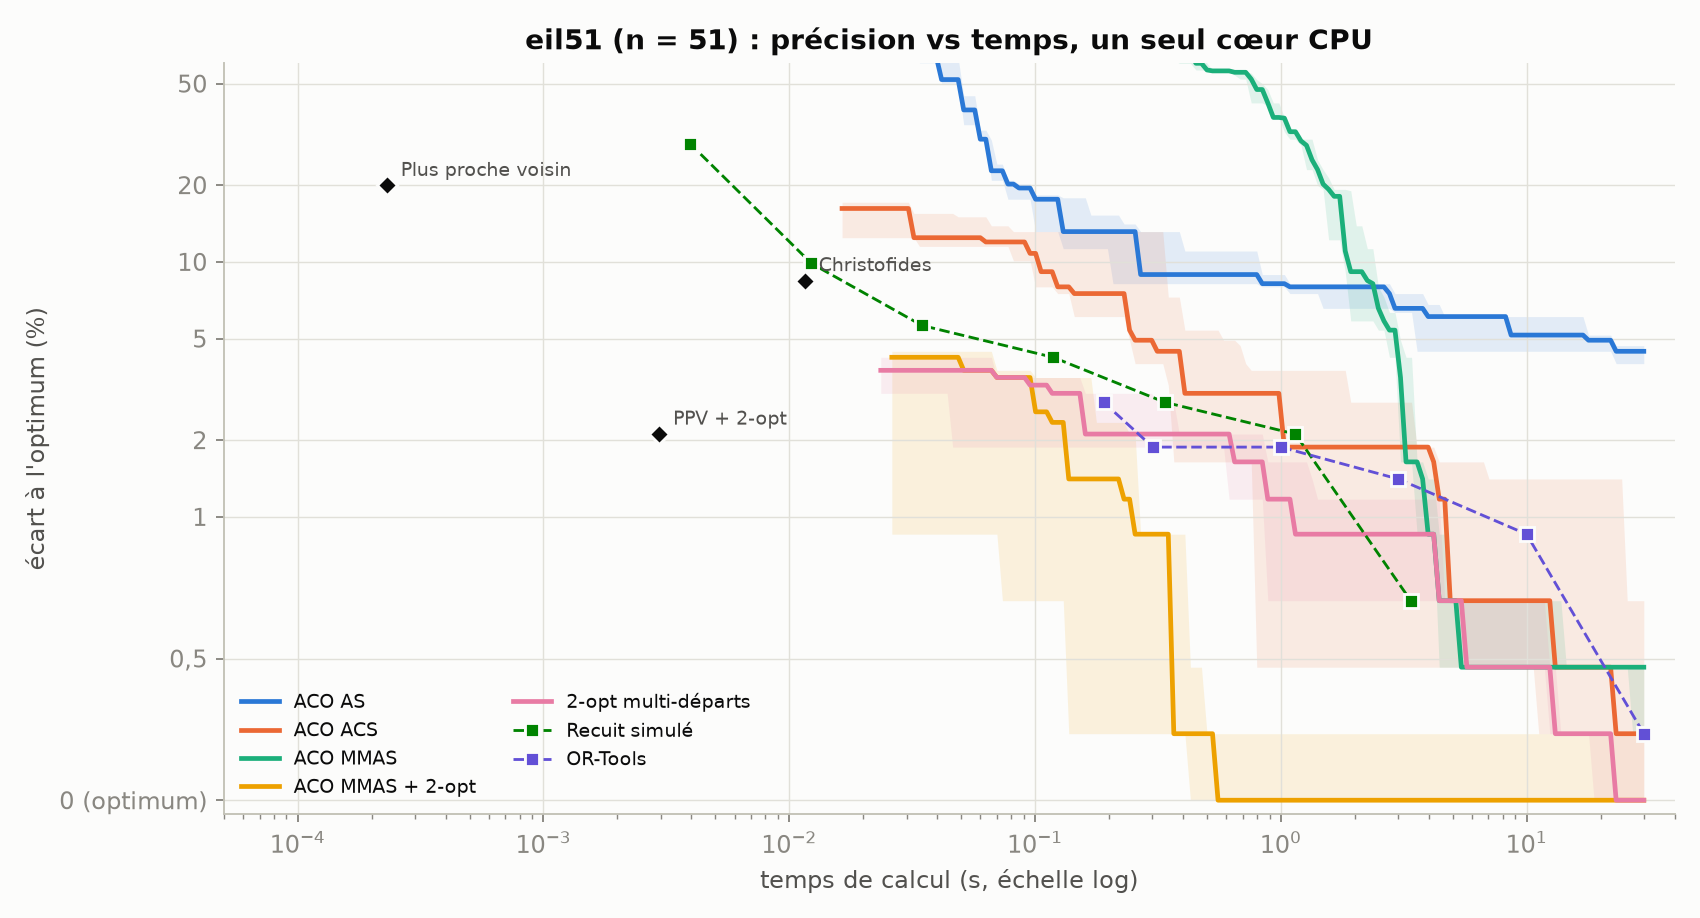
\includegraphics[height=0.84\textheight]{anytime_eil51.png}
\end{frame}

\begin{frame}[fragile]{Annexe : reproduire les résultats}
  \small
  Code : \texttt{github.com/BalboniIvanoWacheQuentin/using-ACO-for-TSP}
  \begin{itemize}
    \item \texttt{python accuracy\_time.py} : complexité et précision vs temps
          (\texttt{results/complexity.csv}, \texttt{anytime.csv})
    \item \texttt{python plot\_accuracy\_time.py} : figures et tableau par budget
    \item \texttt{python experiments.py} : étude des paramètres de l'ACO
    \item \texttt{python slides/make\_figures.py} : figures complémentaires
    \item \texttt{streamlit run streamlit.py} : démonstration interactive (aussi en ligne :
          \nolinkurl{using-aco-for-tsp-faqcu8kd7htkggervtpugk.streamlit.app})
  \end{itemize}
\end{frame}

\end{document}
